\chapter{RESULTS OF STYLE BASED TONE MAPPING}
\label{app:results}
\rotatebox{90}{\begin{minipage}{0.74\textheight}
    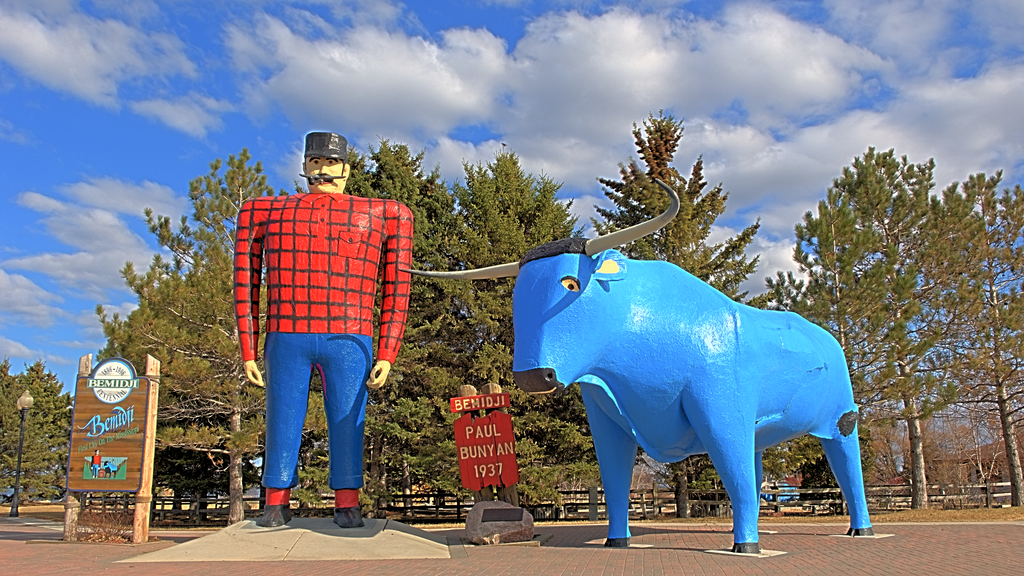
\includegraphics[width=\textwidth]{figures/chapter5/style_based/PaulBunyan_hdrcandy_v1.png}
    \captionof{figure}{High resolution version of Figure~\ref{FigStyle}(a).}
    \label{fig:PropProf}
\end{minipage}}

%\begin{sidewaysfigure}
%\begin{center}
%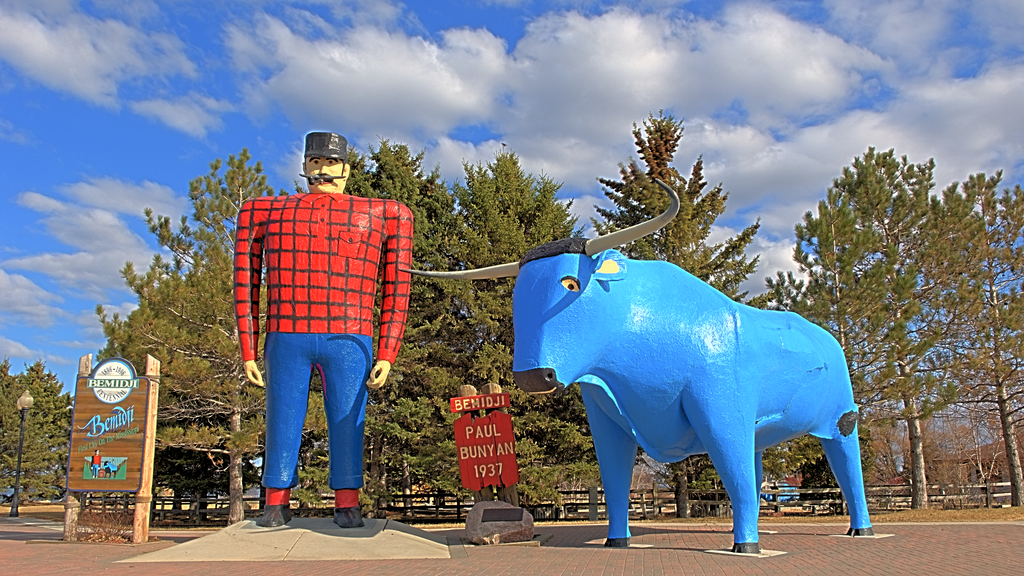
\includegraphics[width=\textwidth]{figures/chapter5/style_based/PaulBunyan_hdrcandy_v1.png}
%\caption{Manually tone mapped calibration images for \emph{candy} style.}
%\end{center}
%\end{sidewaysfigure}

\begin{sidewaysfigure}
\begin{center}
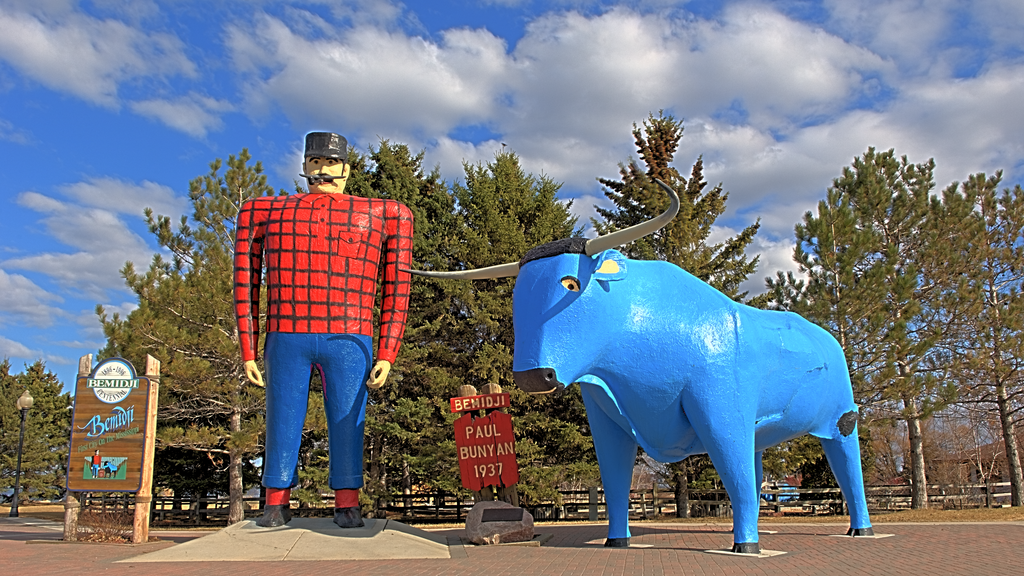
\includegraphics[width=\textwidth]{figures/chapter5/style_based/PaulBunyan_hdrcandy_v2.png}
\caption{High resolution version of Figure~\ref{FigStyle}(b).}
\end{center}
\end{sidewaysfigure}

\begin{sidewaysfigure}
\begin{center}
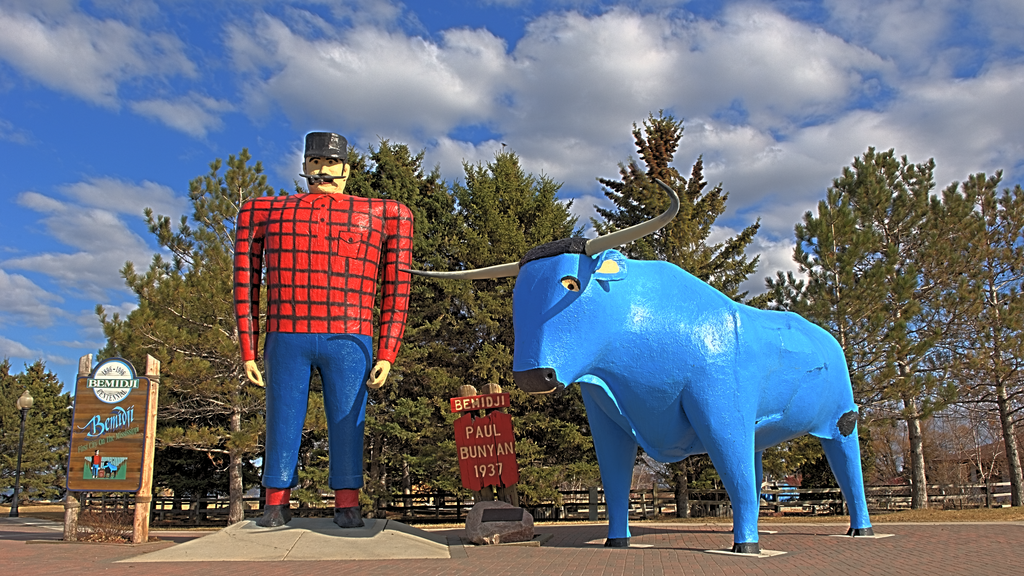
\includegraphics[width=\textwidth]{figures/chapter5/style_based/PaulBunyan_hdrcandy_w0_1.png}
\caption{High resolution version of Figure~\ref{FigStyle}(c).}
\end{center}
\end{sidewaysfigure}

\begin{sidewaysfigure}
\begin{center}
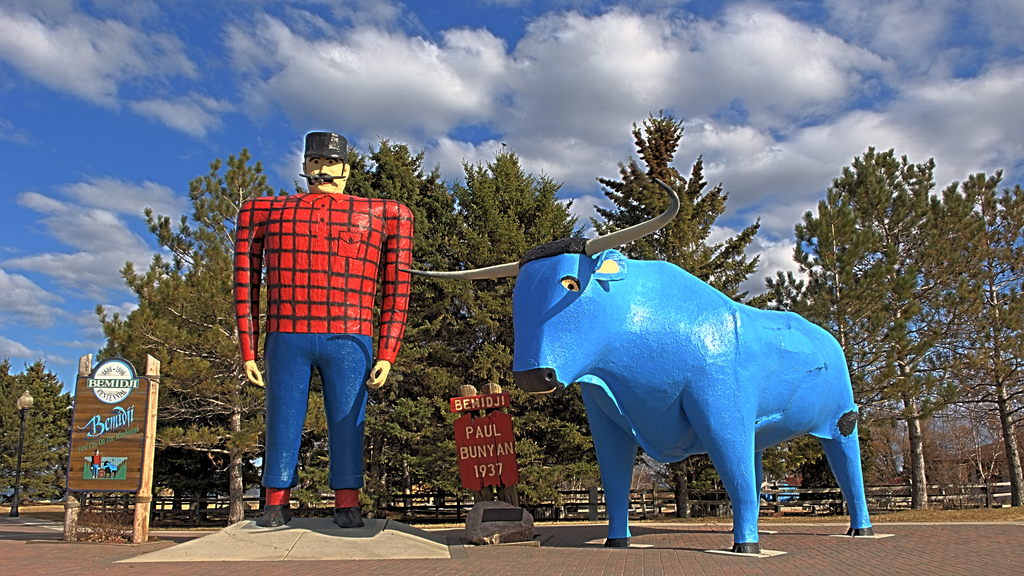
\includegraphics[width=\textwidth]{figures/chapter5/style_based/PaulBunyan_hdrcandy_w0_w1_w2.png}
\caption{High resolution version of Figure~\ref{FigStyle}(d).}
\end{center}
\end{sidewaysfigure}

\begin{sidewaysfigure}
\begin{center}
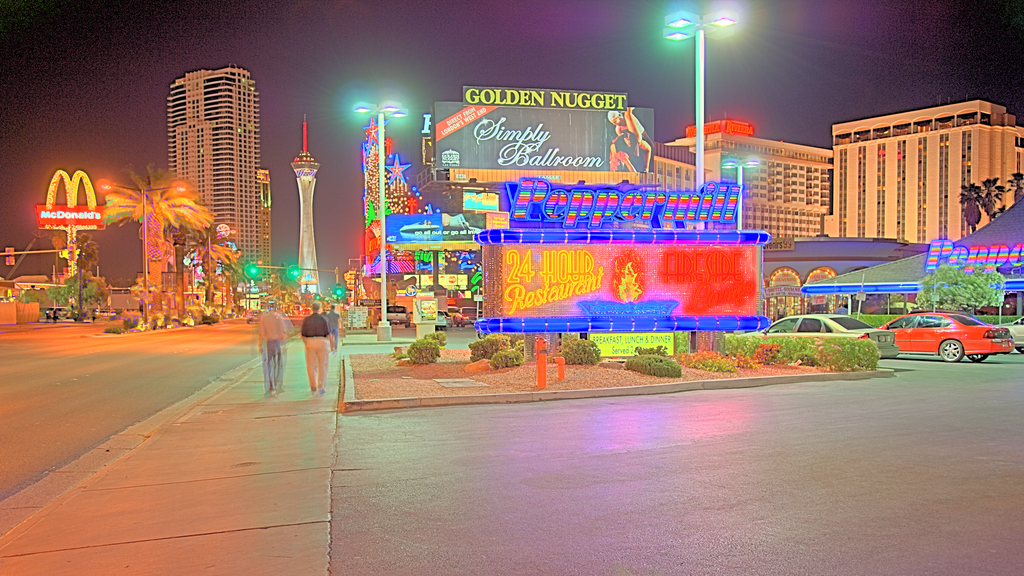
\includegraphics[width=\textwidth]{figures/chapter5/style_based/Peppermill_hdrcandy_v1.png}
\caption{High resolution version of Figure~\ref{FigStyle}(e).}
\end{center}
\end{sidewaysfigure}

\begin{sidewaysfigure}
\begin{center}
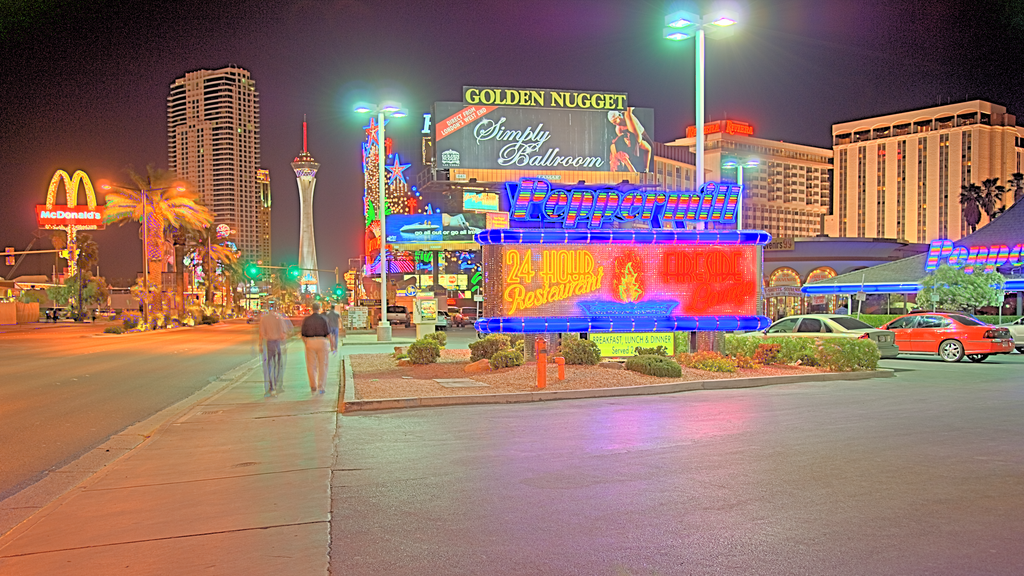
\includegraphics[width=\textwidth]{figures/chapter5/style_based/Peppermill_hdrcandy_v2.png}
\caption{High resolution version of Figure~\ref{FigStyle}(f).}
\end{center}
\end{sidewaysfigure}

\begin{sidewaysfigure}
\begin{center}
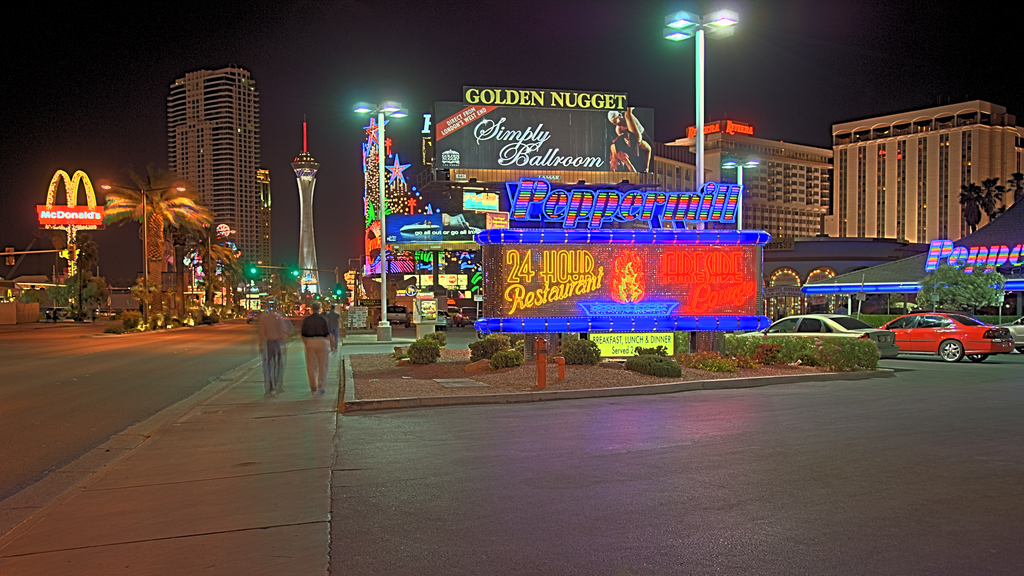
\includegraphics[width=\textwidth]{figures/chapter5/style_based/Peppermill_hdrcandy_w0_1.png}
\caption{High resolution version of Figure~\ref{FigStyle}(g).}
\end{center}
\end{sidewaysfigure}

\begin{sidewaysfigure}
\begin{center}
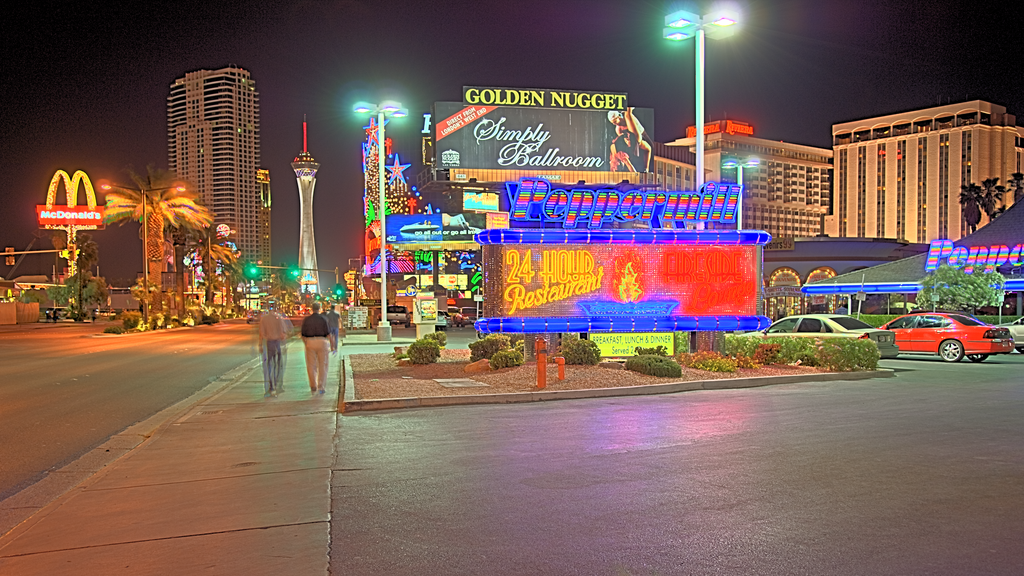
\includegraphics[width=\textwidth]{figures/chapter5/style_based/Peppermill_hdrcandy_w0_w1_w2.png}
\caption{High resolution version of Figure~\ref{FigStyle}(h).}
\end{center}
\end{sidewaysfigure}